\documentclass[a4paper]{scrartcl}
\usepackage[english]{babel}
\usepackage[top=2cm,bottom=3cm,left=2.5cm,right=2.5cm]{geometry}
\usepackage[colorlinks=true, allcolors=black]{hyperref}
\usepackage{wrapfig} %문단 내 이미지 삽입
\usepackage{graphicx} %색상
\usepackage{overpic}
\usepackage[normalem]{ulem}%취소선
\usepackage{array} %표
\usepackage{mdframed, tcolorbox} %글상자
\usepackage[yyyymmdd]{datetime}
	\renewcommand{\dateseparator}{--}
\usepackage{amsmath, amsfonts, amssymb, bm} %수식
	\DeclareMathOperator{\arccsc}{arccsc}
	\DeclareMathOperator{\arcsec}{arcsec}
	\DeclareMathOperator{\arccot}{arccot}
	\DeclareMathOperator{\csch}{csch}
	\DeclareMathOperator{\sech}{sech}
	\DeclareMathOperator{\arcsinh}{arcsinh}
	\DeclareMathOperator{\arccosh}{arccosh}
	\DeclareMathOperator{\arctanh}{arctanh}
	\DeclareMathOperator{\arccsch}{arccsch}
	\DeclareMathOperator{\arcsech}{arcsech}
	\DeclareMathOperator{\arccoth}{arccoth}
	
	\DeclareMathOperator{\meter}{m}
	\DeclareMathOperator{\cm}{cm}
	\DeclareMathOperator{\mm}{mm}
	\DeclareMathOperator{\mum}{\mu m}
	\DeclareMathOperator{\newton}{N}
	\DeclareMathOperator{\kn}{kN}
	\DeclareMathOperator{\kgf}{kgf}
	\DeclareMathOperator{\pa}{Pa}
	\DeclareMathOperator{\kpa}{kPa}
	\DeclareMathOperator{\mpa}{MPa}
	\DeclareMathOperator{\gpa}{GPa}
	\DeclareMathOperator{\npm}{N/m}
	\DeclareMathOperator{\knpm}{kN/m}
	\DeclareMathOperator{\kph}{km/h}
	\DeclareMathOperator{\mps}{m/s}
	\DeclareMathOperator{\tkph}{kph}
	\DeclareMathOperator{\tmps}{mps}
	\DeclareMathOperator{\mpss}{m/s^2}
	\DeclareMathOperator{\dgr}{\!^\circ}
	\DeclareMathOperator{\cel}{\!^\circ C}
	\DeclareMathOperator{\kg}{kg}
	\DeclareMathOperator{\kgpcm}{kg/m^3}
	\DeclareMathOperator{\nm}{N\cdot m}
	\DeclareMathOperator{\knm}{kN\cdot m}
	\DeclareMathOperator{\kw}{kW}
	\DeclareMathOperator{\kwh}{kWh}
	\DeclareMathOperator{\mmhg}{mmHg}
	\DeclareMathOperator{\snd}{s}
\usepackage{polynom} %나눗셈 필산
\usepackage{cancel} %수식 약분선
\usepackage{titlesec} %섹션 이름 변경
	\titlespacing*{\section}{3mm}{0mm}{1mm}
	\titleformat{\section}{\bfseries\large}{}{0ex}{}
\usepackage{kotex} %한글

\newcommand{\prob}[2]{\section{#1}\begin{mdframed}#2\end{mdframed}}

\newlength{\picwidth}
\newcommand{\probpic}[4]{
	\setlength{\picwidth}{145mm}\addtolength{\picwidth}{-#3}\section{#1}\begin{mdframed}\begin{tabular}{m{#3}m{\picwidth}}
	\includegraphics[width = #3]{#2} & #4\end{tabular}\end{mdframed}
	}

\title{\vspace{100pt}\Huge{HW3}}
\author{
	2025-2 구조역학(박성훈 교수님)\\[10pt]
	Problem 9.1, 9.3, 9.10, 9.16, 9.20, 9.67, 9.72, 9.76\\[110pt]
	}
\date{\today}

\begin{document}
	
\renewcommand*{\titlepagestyle}{empty}
\maketitle

\vspace{60pt}

\begin{center}
	\includegraphics[width=0.45\textwidth]{SSU symbol KR-EN.jpg}
\end{center}

\newpage\setcounter{page}{1}

\setlength{\parindent}{0pt}

\noindent\textbf{\textsf{In the following problems, assume that the flexural rigidity $EI$ of each beam is constant.}}\\

\prob{Problem 9.1 and 9.3}{For the loading shown, determine ($a$) the equation of the elastic curve for the cantilever beam $AB$, ($b$) the deflection at the free end, ($c$) the slope at the free end.\begin{center}\includegraphics[width = 65mm]{img/p9.1.png}\qquad\includegraphics[width = 65mm]{img/p9.3.png}\end{center}}
	\begin{align*}
		&\text{Prob. 9.1}\quad\blacktriangledown && \text{Prob. 9.3}\quad\blacktriangledown\\[10pt]
		&+\circlearrowleft\sum M|_A = -PL + M_A = 0 && +\circlearrowleft\sum M|_B = wL\left(\frac{L}{2}\right) - M_B = 0\\
		&\phantom{.}\quad\Rightarrow\quad M_A = PL\;(\circlearrowleft) &&\phantom{.}\quad\Rightarrow\quad M_B = \frac{wL^2}{2}\;(\circlearrowright)\\
		&+\uparrow\sum F_y = R_A - P = 0 && +\uparrow\sum F_y = R_B - wL = 0\\
		&\phantom{.}\quad\Rightarrow\quad R_A = P\;(\uparrow) && \phantom{.}\quad\Rightarrow\quad R_B = wL\;(\uparrow)\\
		&V(x) = P\;\Rightarrow\; M(x) = Px - PL && V(x) = -wx\;\Rightarrow\; M(x) = -\frac{w}{2}x^2\\
		&EI\theta(x) = \frac{P}{2}x^2 - PLx + c_1 && EI\theta(x) = -\frac{w}{6}x^3 + c_1\\
		&\theta(0) = 0\quad\Rightarrow\quad c_1 = 0 && \theta(L) = 0\quad\Rightarrow\quad c_1 = \frac{wL^3}{6}\\
		&EIy(x) = \frac{P}{6}x^3 - \frac{PL}{2}x^2 + c_2 && EIy(x) = -\frac{w}{24}x^4 + \frac{wL^3}{6}x + c_2\\
		&y(0) = 0\quad\Rightarrow\quad c_2 = 0 && y(L) = 0\quad\Rightarrow\quad c_2 = -\frac{wL^4}{8}\\
		&\theta(x) = \frac{P}{2EI}(x^2 - 2Lx) && \theta(x) = -\frac{w}{6EI}(x^3 - L^3)\\
		&y(x) = \frac{P}{6EI}(x^3 - 3Lx^2)\quad\blacktriangleleft\;(a) && y(x) = -\frac{w}{24EI}(x^4 - 4L^3x + 3L^4)\;\blacktriangleleft\;(a)\\
		&y(L) = -\frac{PL^3}{3EI}\quad\blacktriangleleft\;(b) && y(0) = -\frac{wL^4}{8EI}\quad\blacktriangleleft\;(b)\\
		&\theta(L) = -\frac{PL^2}{2EI}\quad\blacktriangleleft\;(c) && \theta(0) = \frac{wL^3}{6EI}\quad\blacktriangleleft\;(c)
	\end{align*}

\newpage

\probpic{Problem 9.10}{img/p9.10.png}{67mm}{Knowing that beam $AB$ is a W130$\times$23.8 rolled shape and that $P=50\kn$. $L= 1.25\meter$, and $E = 200\gpa$, determine ($a$) the slope at $A$. ($b$) the deflection at $C$.\newline\newline * $I = 8.91\times10^6\mm^4\;\cdots\;$ appendix E}
	\begin{align*}
		&+\circlearrowleft\sum M|_A = -\frac{PL}{2} + R_BL = 0,\quad R_B = \frac{P}{2}\;(\uparrow)\\
		&+\circlearrowleft\sum F_y = -P + R_A + R_B = 0,\quad R_A = \frac{P}{2}\;(\uparrow)\\
		&V(x) = \left\{\begin{array}{ll}\cfrac{P}{2} & \left(0\leq x \leq \cfrac{L}{2}\right)\\[20pt]-\cfrac{P}{2} & \left(\cfrac{L}{2}\leq x \leq L\right)\end{array}\right.\quad\Rightarrow\quad M(x) = \left\{\begin{array}{ll}\cfrac{P}{2}x & \left(0\leq x \leq \cfrac{L}{2}\right)\\[20pt]-\cfrac{P}{2}(x-L) & \left(\cfrac{L}{2}\leq x \leq L\right)\end{array}\right.\\
		&EI\theta(x) = \left\{\begin{array}{ll}\cfrac{P}{4}x^2 + c_1 & ('')\\[20pt]-\cfrac{P}{4}(x-L)^2 + c_2& ('')\end{array}\right.\quad\Rightarrow\quad EIy(x) = \left\{\begin{array}{ll}\cfrac{P}{12}x^3 + c_1x + c_3& ('')\\[20pt]-\cfrac{P}{12}(x-L)^3 + c_2x + c_4& ('')\end{array}\right.\\
		&\theta\left(\frac{L}{2}\right) = 0\quad\Rightarrow\quad EI\theta\left(\frac{L}{2}\right) = \frac{P}{4}\left(\frac{L}{2}\right)^2 + c_1 = -\frac{P}{4}\left(-\frac{L}{2}\right)^2 + c_2 = 0\\
		&\Rightarrow\quad c_1 = -\frac{PL^2}{16},\quad c_2 = \frac{PL^2}{16}\\
		&y(0) = 0\quad\Rightarrow\quad EIy(0) = c_3 = 0\\
		&y(L) = 0\quad\Rightarrow\quad EIy(L) = c_2L + c_4 = 0,\quad c_4 = -c_2L = -\frac{PL^3}{16}\\
		&\theta(0) = \frac{c_1}{EI} = -\frac{PL^2}{16EI} = -2.74\times10^{-3}\quad\blacktriangleleft\quad(a)\\
		&y\left(\frac{L}{2}\right) = \frac{1}{EI}\left\{\frac{P}{12}\left(\frac{L}{2}\right)^3 - \frac{PL^2}{16}\left(\frac{L}{2}\right)\right\} = -\frac{PL^3}{48EI} = -1.142\mm\quad\blacktriangleleft\quad(b)
	\end{align*}

\newpage

\probpic{Problem 9.16}{img/p9.16.png}{70mm}{For the beam and loading shown, determine the deflection at point $C$, Use $E = 200\gpa$\newline\newline from appendix E : $I = 9.20\times10^6\mm^4$}
	\begin{align*}
		&+\circlearrowleft\sum M|_A = -P\cdot\frac{L}{3} + R_B L = 0,\quad R_B = \frac{P}{3}\uparrow\\
		&+\uparrow\sum F_y = R_A + R_B - P = 0,\quad R_A = \frac{2P}{3}\uparrow\\
		&V(x) = \left\{\begin{array}{ll}
			\cfrac{2P}{3} & \left(0\leq x \leq a\right)\\
			-\cfrac{P}{3} & \left(a< x \leq L\right)
		\end{array}\right.\quad\Rightarrow\quad
		M(x) = \left\{\begin{array}{ll}
			\cfrac{2P}{3}x & ('')\\
			-\cfrac{P}{3}x + \cfrac{PL}{3} = -\cfrac{P}{3}(x-L) & ('')
		\end{array}\right.\\
		&EI\theta(x)
		= \left\{\begin{array}{l}
			\cfrac{P}{3}x^2 + c_1\\
			-\cfrac{P}{6}(x-L)^2 + c_2
		\end{array}\right.\quad\Rightarrow\quad
		EIy(x)
		= \left\{\begin{array}{l}
			\cfrac{P}{9}x^3 + c_1x + c_3\\
			-\cfrac{P}{18}(x-L)^3 + c_2x + c_4
		\end{array}\right.
	\end{align*}
	The boundary conditions are $y(0) = y(L) = 0$, $\theta_1(L/3) = \theta_2(L/3)$ and $y_1(L/3) = y_2(L/3)$.
	\begin{align*}
		&EIy(0) = c_3 = 0\\
		&EIy(L) = c_2L + c_4 = 0\tag{1}\\
		&EI\theta\left(\frac{L}{3}\right) = \frac{PL^2}{27} + c_1 = -\frac{2PL^2}{27} + c_2\tag{2}\\
		&EIy\left(\frac{L}{3}\right) = \frac{PL^3}{243} + c_1L + \cancelto{0}{c_3} = \frac{4PL^3}{243} + c_2\frac{L}{3} + c_4\tag{3}
	\end{align*}
	We can make a series of equations with equations (1), (2) and (3).
	\begin{align*}
		&\begin{array}{lllll}
			& Lc_2 & +c_4 & = 0 &\quad(1)\\[10pt]
			c_1 & -c_2 & & = -\cfrac{PL^2}{9} &\quad(2)\\[10pt]
			\cfrac{L}{3}c_1 & -\cfrac{L}{3} c_2 & -c_4 & = \cfrac{PL^3}{81} &\quad(3)
		\end{array}\quad\Rightarrow\quad
		\left(\begin{array}{ccc|c}
			0 & L & 1 & 0\\[5pt]
			1 & -1 & 0& -\frac{PL^2}{9}\\[5pt]
			\frac{L}{3} & -\frac{L}{3} & -1 & \frac{PL^3}{81}
		\end{array}\right)
	\end{align*}
	Use a scientific calculator. \framebox{\texttt{MODE}}$\,\to\,$\framebox{\texttt{5}} (Equations)
	\begin{align*}
		&c_1 = -\frac{5PL^2}{81},\quad c_2 = \frac{4PL^2}{81},\quad c_4 = -\frac{4PL^3}{81}\\
		&\theta(x)
		= \left\{\begin{array}{l}
			\cfrac{P}{81EI}\left(27x^2 - 5L^2\right)\\
			-\cfrac{P}{162EI}\left(27x^2-54Lx+19L^2\right)
		\end{array}\right.,\quad
		y(x)
		= \left\{\begin{array}{l}
			\cfrac{P}{81EI}\left(9x^3 -5L^2x\right)\\
			-\cfrac{P}{162EI}\left(9x^3 - 27Lx^2 + 19L^2x -L^3\right)
		\end{array}\right.\\[10pt]
		&y\left(\frac{L}{3}\right) = -\frac{4PL^3}{243EI} = -4.83\mm\quad\blacktriangleleft
	\end{align*}
	
\newpage

\probpic{Problem 9.20}{img/p9.20.png}{55mm}{For the beam and loading shown, determine the reaction at the roller support.}

\begin{align*}
	&+\uparrow \sum F_y = R_A - wL + R_B = 0\tag{1}\\
	&+\circlearrowleft \sum M|_B = M_B + wL\cdot\frac{L}{2} - R_AL = 0\tag{2}\\
	&M(0) = 0,\quad M(x) = R_Ax - wx\cdot\frac{x}{2} = -\frac{w}{2}x^2 + R_Ax\\
	&EI\theta(x) = -\frac{w}{6}x^3 + \frac{R_A}{2}x^2 + c_1\\
	&\theta(L) = 0\quad\Rightarrow\quad EI\theta(L) = -\frac{wL^3}{6} + \frac{R_A L^2}{2}+ c_1 = 0\tag{3}\\
	&EIy(x) = -\frac{w}{24}x^4 + \frac{R_A}{6}x^3 +c_1x + c_2\\
	&y(0) = 0\quad\Rightarrow\quad EIy(0) = c_2 = 0\\
	&y(L) = 0\quad\Rightarrow\quad EIy(L) = -\frac{wL^4}{24} + \frac{R_AL^3}{6} + c_1L = 0\tag{4}\\[10pt]
	&\begin{array}{lllll}
		-LR_A & +M_B &  & = -\cfrac{wL^2}{2} &\quad(2)\\[10pt]
		\cfrac{L^2}{2}R_A & & +c_1 & = \cfrac{wL^3}{6} &\quad(3)\\[10pt]
		\cfrac{L^3}{6}R_A & & +Lc_1 & = \cfrac{wL^4}{24} &\quad(4)
	\end{array}\quad\Rightarrow\quad
	\left(\begin{array}{ccc|c}
		-L & 1 & 0 & -\frac{wL^2}{2}\\[5pt]
		\frac{L^2}{2} & 0 & 1& \frac{wL^3}{6}\\[5pt]
		\frac{L^3}{6} & 0 & L & \frac{wL^4}{24}
	\end{array}\right)\\
	&R_A = \frac{3wL}{8}\;(\uparrow)\quad\blacktriangleleft\quad,\quad M_B = -\frac{wL^2}{8},\quad c_1 = -\frac{wL^3}{48}\\
	&\text{From the eq.(1),}\quad R_B = wL - R_A = \frac{5wL}{8}
\end{align*}


\newpage

\noindent\textbf{\textsf{Use the method of superposition to solve the following problems and assume that the flexural rigidity $EI$ of each beam is constant.}}\\

\probpic{Problem 9.67}{img/p9.67.png}{55mm}{For the cantilever beam and loading shown, determine the slope and deflection at the free end.}

From the solution of prob.9.1, the slope and deflection of the end point of a cantilever beam are
\begin{align*}
	&\theta_\text{end} = \pm\frac{PL^2}{2EI},\quad y_\text{end} = \pm\frac{PL^3}{3EI}
\end{align*}
Case 1,\\[10pt]
\begin{tabular}{m{65mm}m{100mm}}
	\includegraphics[width = 55mm]{img/fig001.png}
	&
	$\theta_{A1} = \cfrac{PL^2}{2EI},\quad y_{A1} = -\cfrac{PL^3}{3EI}$\\
	\quad
\end{tabular}

Case 2,\\[10pt]
\begin{tabular}{m{65mm}m{100mm}}
	\includegraphics[width = 55mm]{img/fig002.png}
	&
	$\theta_{B2} = \cfrac{(2P)(\frac{L}{2})^2}{2EI} = \cfrac{PL^2}{4EI}$\newline\newline
	$y_{B2} = -\cfrac{(2P)(\frac{L}{2})^3}{3EI} = -\cfrac{PL^3}{12EI}$
\end{tabular}
\begin{align*}
	&\theta_{A2} = \theta_{B2} = \frac{PL^2}{4EI}\\
	&y_{A2} = y_{B2} + \theta_{B2}\times\left(-\frac{L}{2}\right) = -\frac{5PL^3}{24EI}\\
	&\theta_A = \theta_{A1} + \theta_{A2} = \frac{3PL^2}{4EI}\quad\blacktriangleleft\\
	&y_A = y_{A1} + y_{A2} = -\frac{13PL^3}{24EI}\quad\blacktriangleleft
\end{align*}

\newpage

\probpic{Problem 9.72}{img/p9.72.png}{60mm}{For the beam and loading loadin shown, determine ($a$) the deflection at point $C$, ($b$) the slope at end $A$.}
From the solution of prob.9.16,
\begin{align*}
	&\theta(0) = -\frac{5PL^2}{81EI},\quad \theta(L) = \frac{4PL^2}{81EI}\\
	&y\left(\frac{L}{3}\right) = -\frac{4PL^3}{243EI},\quad y\left(\frac{2L}{3}\right) = -\frac{7PL^3}{486EI}
\end{align*}
Case 1,\\
\begin{tabular}{m{65mm}m{100mm}}
	\includegraphics[width = 60mm]{img/fig003.png}
	&
	$\displaystyle \theta_{A1} = -\frac{5PL^2}{81EI},\quad y_{C1} = -\frac{7PL^3}{486EI}$\\
	\quad
\end{tabular}

Case 2,\\
\begin{tabular}{m{65mm}m{100mm}}
	\includegraphics[width = 60mm]{img/fig004.png}
	&
	$\displaystyle \theta_{A2} = \frac{4PL^2}{81EI},\quad y_{C2} = \frac{4PL^3}{243EI}$
\end{tabular}
\begin{align*}
	&y_{C} = y_{C1} + y_{C2} = \frac{PL^3}{486EI}\quad\blacktriangleleft\quad(a)\\
	&\theta_{A} = \theta_{A1} + \theta_{A2} = -\frac{PL^2}{81EI}\quad\blacktriangleleft\quad(b)
\end{align*}

\newpage

\probpic{Problem 9.76}{img/p9.76.png}{65mm}{For the cantilever beam and loading shown, determine the slope and deflection at point $B$. Use $E = 200\gpa$.}
\begin{align*}
	&I = \frac{\pi}{4}(0.022)^4\meter^4 = 1.839842\times10^{-7}\meter^4\\
	&\text{let}\quad w = 2.6\knpm,\quad P = 500\newton,\quad L = 1\meter
\end{align*}
Case 1,\\
\begin{tabular}{m{53mm}m{100mm}}
	\includegraphics[width = 50mm]{img/fig005.png}
	&
	From the solution of prob.9.3,\newline\newline
	$\displaystyle \theta_{B1} = -\frac{w\left(\frac{3L}{4}\right)^3}{6EI} = -\frac{9wL^3}{128EI}$\newline\newline
	$\displaystyle y_{B1} = -\frac{w\left(\frac{3L}{4}\right)^4}{8EI} = -\frac{81wL^4}{2048EI}$\\
	\quad
\end{tabular}

Case 2,\\
\begin{tabular}{m{53mm}m{100mm}}
	\includegraphics[width = 50mm]{img/fig006.png}
	&
	From the solution of prob.9.1,\newline\newline
	$\displaystyle \theta_{B2} = \theta\left(\frac{3L}{4}\right) = -\frac{15PL^2}{32EI}$\newline\newline
	$\displaystyle y_{B2} = y\left(\frac{3L}{4}\right) = -\frac{27PL^3}{128EI}$
\end{tabular}
\begin{align*}
	&\theta_{B} = \theta_{B1} + \theta_{B2} = -\frac{9wL^3}{128EI}-\frac{15PL^2}{32EI} = -0.01134\quad\blacktriangleleft\\
	&y_{B} = y_{B1} + y_{B2} = -\frac{81wL^4}{2048EI} -\frac{27PL^3}{128EI} = -5.66\mm\quad\blacktriangleleft
\end{align*}


\end{document}